
\documentclass{article}	

\ifdefined\HCode
\def\pgfsysdriver{pgfsys-tex4ht.def}
\fi
\usepackage{tikz,graphicx}
\usetikzlibrary{external}

\tikzset{
    png copy/.style={
        external/system call={
            pdflatex \tikzexternalcheckshellescape -halt-on-error -interaction=batchmode -jobname "\image" "\texsource";
            convert -density 300 -transparent white "\image.pdf" "\image.png"
        }
    }
}
\tikzset{png copy}

\makeatletter
\@ifpackageloaded{tex4ht}{
\tikzexternalize[mode=only graphics]
\tikzset{png export/.style={/pgf/images/external info,/pgf/images/include external/.code={\includegraphics[width=\pgfexternalwidth,height=\pgfexternalheight]{##1.png}}}}
\tikzset{png export}
}{
\tikzexternalize
\tikzset{pdf export/.style={/pgf/images/external info,/pgf/images/include external/.code={\includegraphics[width=\pgfexternalwidth,height=\pgfexternalheight]{##1.pdf}}}}
\tikzset{pdf export}
}
\makeatother

\usepackage{natbib}
\usepackage{amssymb,amsmath,multicol,subfigure, float, ifthen}
\usepackage{caption}
\usepackage[hmargin=1in, vmargin=1in]{geometry}
\usetikzlibrary{positioning,shapes,arrows,shapes.symbols}
\usetikzlibrary{decorations.pathmorphing}

%\usepackage[nomarkers]{endfloat}

\begin{document}

\subsection{Introduction}
Blah Blah Blah... Blah Blah Blah... Blah Blah Blah... Blah Blah Blah... Blah Blah Blah... Blah Blah Blah... Blah Blah Blah... Blah Blah Blah... Blah Blah Blah... Blah Blah Blah... Blah Blah Blah... Blah Blah Blah... Blah Blah Blah... Blah Blah Blah... Blah Blah Blah... Blah Blah Blah... Blah Blah Blah... Blah Blah Blah... Blah Blah Blah... Blah Blah Blah... Blah Blah Blah... Blah Blah Blah... Blah Blah Blah... Blah Blah Blah... Blah Blah Blah... Blah Blah Blah... Blah Blah Blah... Blah Blah Blah... Blah Blah Blah... 

\begin{table}[H]
\caption{Correlations used in microchannel condenser\label{tab:TheTable}}
\centering
\begin{tabular}{ccc}
\hline 
C1 & C2 & C3 \\ \hline
R1C1 & R1C2 & R1C3 \\ \hline 
\end{tabular} 
\end{table}

A reference to Table \ref{tab:TheTable}.

\section{Equation}

\begin{equation}
a^2+b^2= c^2
\end{equation}

\section{Figure as image}
\begin{figure}[h]
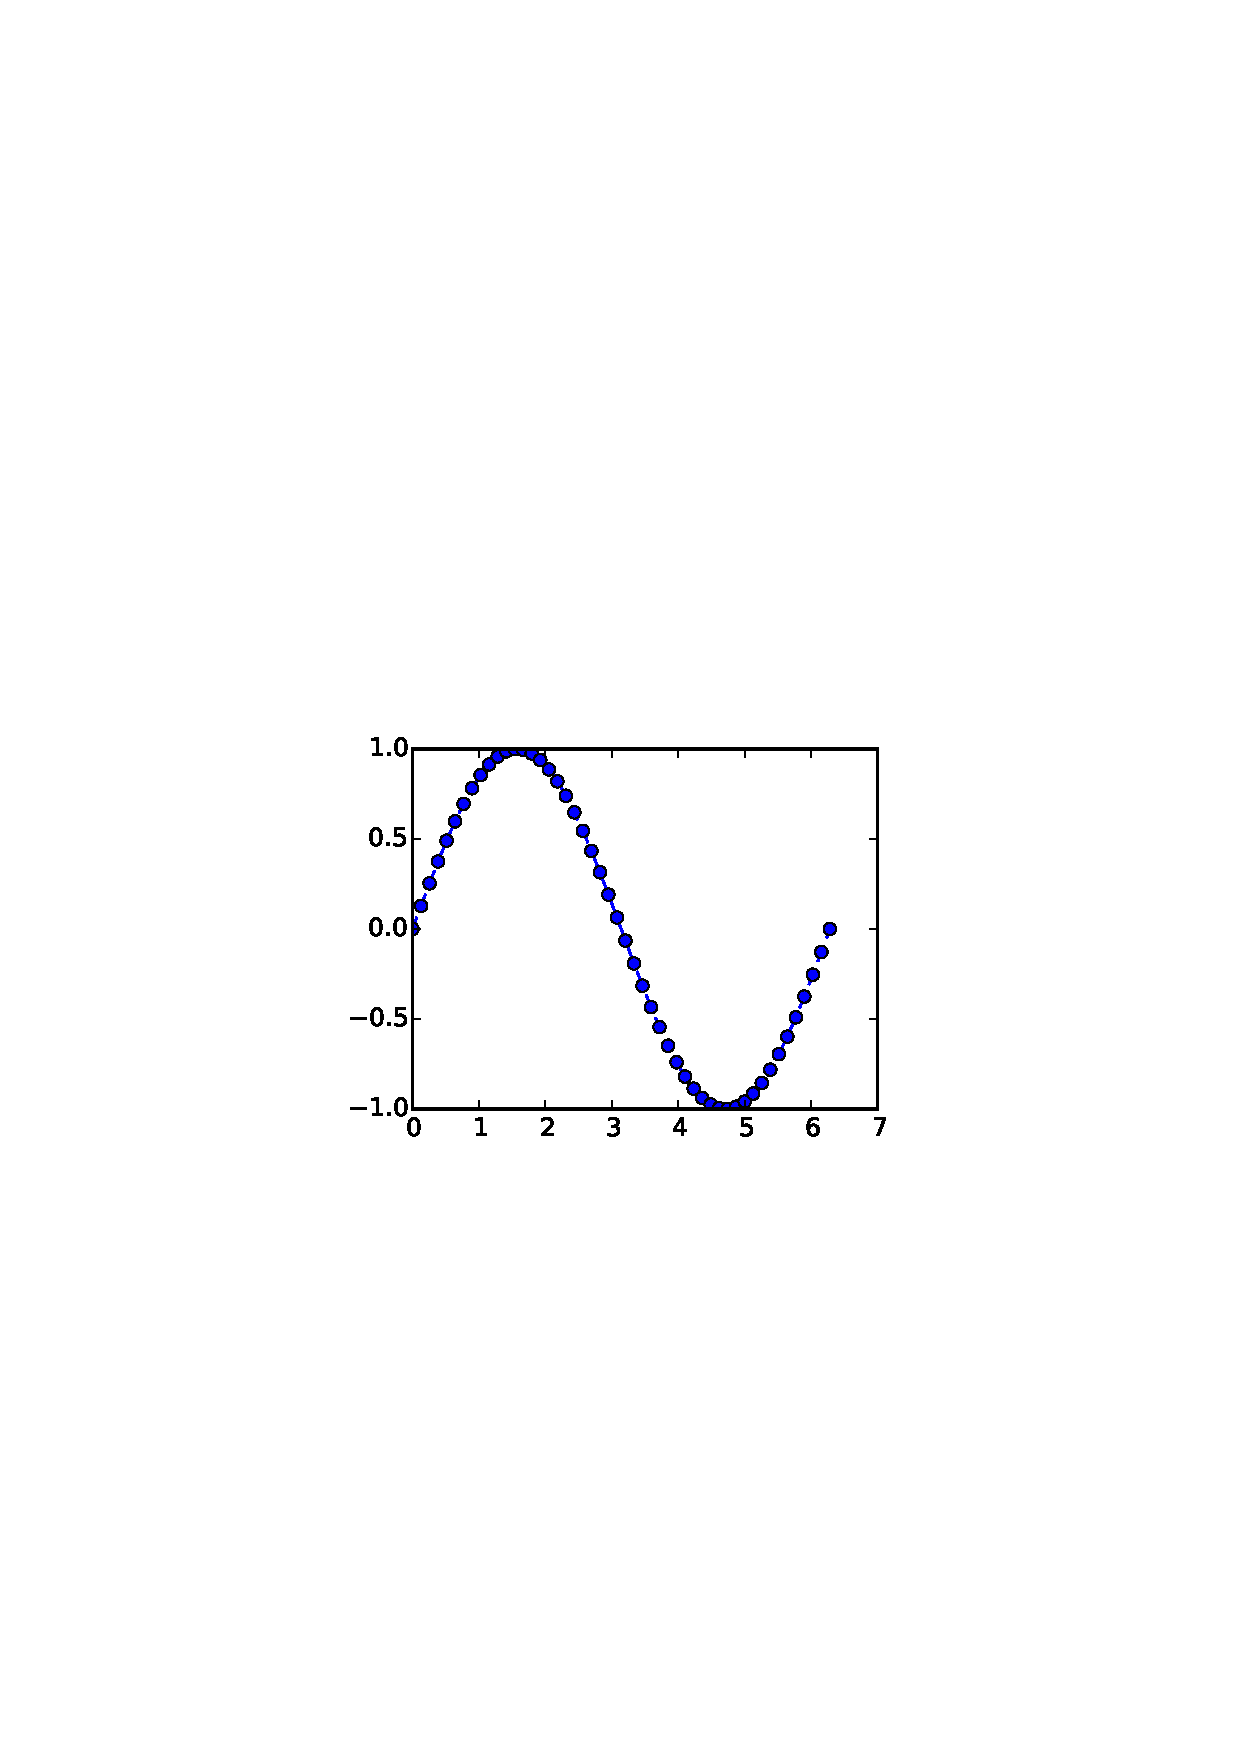
\includegraphics{image.png}
\caption{Figure as image}
\end{figure}

\section{Figure using TikZ}
\begin{figure}[H]
	    
	\centering
	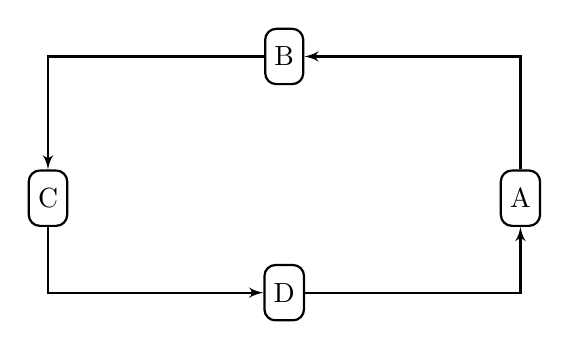
\begin{tikzpicture}[node distance = 1.2cm, auto]
	\tikzstyle{block} = [rectangle, draw, fill=white, text centered, rounded corners, minimum height=2em, thick]
	\tikzstyle{line} = [draw, -latex', thick]
    
	    % Place nodes
	    \node [block, fill = white] (D) {D};
	    \node [block, yshift = 3cm, fill = white] (B) {B};
	    \node [block, yshift = 1.2cm, xshift=3cm, align=center, fill=white] (A) {A};
	    \node [block, yshift = 1.2cm, xshift=-3cm, fill = white,align = center] (C) {C};

	    % Draw edges
	    \path [line] (A) |- (B);
  	    \path [line] (B) -| (C);
  	    \path [line] (C) |- (D);
  	    \path [line] (D) -| (A);
   	    
	\end{tikzpicture}
\caption{Figure using TikZ}
\end{figure}

\end{document}